\documentclass[12pt,a4paper]{paper}
\usepackage[utf8]{inputenc}
\usepackage[english]{babel}
\usepackage{amsmath}
\usepackage{enumitem}
\usepackage{arydshln}
\usepackage{amsfonts}
\usepackage{multirow}
\usepackage{multicol}
\usepackage{vwcol}
\usepackage{amssymb}
\usepackage{tikz}
\usepackage[left=1cm,right=1cm,top=1.5cm,bottom=2cm]{geometry}
\allowdisplaybreaks
\usepackage{Sweave}
\begin{document}
\Sconcordance{concordance:HW5_DanielOsorio.tex:HW5_DanielOsorio.Rnw:%
1 14 1 1 0 41 1 1 11 17 1 1 15 58 1 1 12 42 1 1 7 1 2 8 0 1 2 30 1 1 2 %
1 0 3 1 1 6 18 0 1 2 12 1 1 2 1 0 1 1 9 0 1 2 26 1 1 2 1 0 2 1 1 2 1 0 %
1 1 6 0 1 2 1 0 1 1 6 0 1 1 7 0 1 2 1 1}

\title{GENE638 - Homework 5\\\small{Daniel Osorio - dcosorioh@tamu.edu\\Department of Veterinary Integrative Biosciences\\Texas A\&M University}}
\maketitle

\begin{multicols}{2}
Data:
\begin{center}
\begin{tabular}{|c|c|c|}
\hline
COW&YEAR&TICK COUNT\\
\hline
1&1&80\\
\hline
2&1&70\\
\hline
1&2&86\\
\hline
2&2&72\\
\hline
1&3&92\\
\hline
2&3&78\\
\hline
\end{tabular}
\end{center}
Pedrigree:
\begin{center}
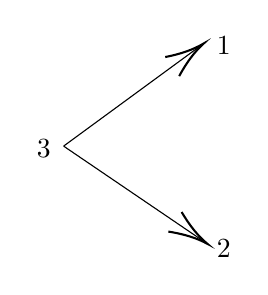
\begin{tikzpicture}[x=1pt,y=1pt,yscale=1.3,xscale=1.3]
\draw    (122.5,43.85) -- (159.89,71.24) ;
\draw [shift={(161.5,72.42)}, rotate = 216.23] [color={rgb, 255:red, 0; green, 0; blue, 0 }  ][line width=0.75]    (10.93,-3.29) .. controls (6.95,-1.4) and (3.31,-0.3) .. (0,0) .. controls (3.31,0.3) and (6.95,1.4) .. (10.93,3.29)   ;

\draw    (122.5,43.85) -- (160.85,17.79) ;
\draw [shift={(162.5,16.67)}, rotate = 505.8] [color={rgb, 255:red, 0; green, 0; blue, 0 }  ][line width=0.75]    (10.93,-3.29) .. controls (6.95,-1.4) and (3.31,-0.3) .. (0,0) .. controls (3.31,0.3) and (6.95,1.4) .. (10.93,3.29)   ;
\draw (117,43.15) node  [align=left] {3};
\draw (167,15.27) node  [align=left] {2};
\draw (167,71.73) node  [align=left] {1};
\end{tikzpicture}
\end{center}
\end{multicols}
\begin{enumerate}
\item Construct the numerator relationship and its inverse
\begin{Schunk}
\begin{Soutput}
     A1   A2  A3  M1  M2
A1 1.00 0.25 0.5 0.5 0.0
A2 0.25 1.00 0.5 0.0 0.5
A3 0.50 0.50 1.0 0.0 0.0
M1 0.50 0.00 0.0 1.0 0.0
M2 0.00 0.50 0.0 0.0 1.0
\end{Soutput}
\begin{Soutput}
   A1 A2   A3   M1   M2
A1  2  0 -1.0 -1.0  0.0
A2  0  2 -1.0  0.0 -1.0
A3 -1 -1  2.0  0.5  0.5
M1 -1  0  0.5  1.5  0.0
M2  0 -1  0.5  0.0  1.5
\end{Soutput}
\end{Schunk}
\item The predicted breeding value of the unidentified parent of animal 1 is $\frac{2}{3}(\hat{A_{1}}-\frac{1}{2}\hat{A_{3}})$ and that for the unidentified parent of animal 2 is $\frac{2}{3}(\hat{A_{2}}-\frac{1}{2}\hat{A_{3}})$. Identify the base generation animals and show that $1'A^{-1}\hat{u} = 0$ is consistent with the sum of breeding values of base generation being 0.
\begin{Schunk}
\begin{Sinput}
> X <- matrix(c(1,1,0,0,0,0,0,0,1,1,0,0,0,0,0,0,1,1), ncol = 3, byrow = FALSE)
> Z <- matrix(c(1,0,1,0,1,0,0,1,0,1,0,1,0,0,0,0,0,0,
+               0,0,0,0,0,0,0,0,0,0,0,0), ncol = 5)
> colnames(Z) <- c("A1","A2","A3","M1","M2")
> colnames(X) <- c("Y1", "Y2", "Y3")
> X1 <- rbind(
+   cbind(t(X) %*% X, t(X) %*% Z), 
+   cbind(t(Z) %*% X, t(Z) %*% Z + Ainv)
+   )
> y <- c(80,70,86,72,92,78)
> Y1 <- c(t(X) %*% y,t(Z) %*% y)
> u <- round(solve(X1) %*% Y1,2)
> rep(1,5) %*% (Ainv %*% u[4:8])
\end{Sinput}
\begin{Soutput}
              [,1]
[1,] -1.776357e-15
\end{Soutput}
\end{Schunk}
\item Write the data in general matrix terms $y = X\beta + Zu + e$ for the model $Y_{ij} = \text{Year}_{i} + \text{Animal}_{j} + e_{ij}$ where $\text{Year}_{i} = \mu + \text{Year}_{i}$. Include animal $3$ in $\hat{u}$ as in (2)
\begin{Schunk}
\begin{Sinput}
> X
\end{Sinput}
\begin{Soutput}
     Y1 Y2 Y3
[1,]  1  0  0
[2,]  1  0  0
[3,]  0  1  0
[4,]  0  1  0
[5,]  0  0  1
[6,]  0  0  1
\end{Soutput}
\begin{Sinput}
> Z[,1:3]
\end{Sinput}
\begin{Soutput}
     A1 A2 A3
[1,]  1  0  0
[2,]  0  1  0
[3,]  1  0  0
[4,]  0  1  0
[5,]  1  0  0
[6,]  0  1  0
\end{Soutput}
\end{Schunk}
\item Assuming $R=I\sigma^{2}_{e}$ and $G = A\sigma^{2}_{a}$ and $\lambda = \frac{\sigma^{2}_{e}}{\sigma^{2}_{a}} = 3$, write the MME for model in (3)
\begin{Schunk}
\begin{Sinput}
> lambda <- 3
> Z <- Z[,1:3]
> Ainv <- solve(A[1:3,1:3])
> Z
\end{Sinput}
\begin{Soutput}
     A1 A2 A3
[1,]  1  0  0
[2,]  0  1  0
[3,]  1  0  0
[4,]  0  1  0
[5,]  1  0  0
[6,]  0  1  0
\end{Soutput}
\begin{Sinput}
> X1 <- rbind(
+   cbind(t(X) %*% X, t(X) %*% Z),
+   cbind(t(Z) %*% X, t(Z) %*% Z + Ainv*lambda)
+   )
> y <- c(80,70,86,72,92,78)
> Y1 <- c(t(X) %*% y,t(Z) %*% y)
> X1
\end{Sinput}
\begin{Soutput}
   Y1 Y2 Y3            A1            A2 A3
Y1  2  0  0  1.000000e+00  1.000000e+00  0
Y2  0  2  0  1.000000e+00  1.000000e+00  0
Y3  0  0  2  1.000000e+00  1.000000e+00  0
A1  1  1  1  7.000000e+00  1.249001e-16 -2
A2  1  1  1  4.440892e-17  7.000000e+00 -2
A3  0  0  0 -2.000000e+00 -2.000000e+00  5
\end{Soutput}
\begin{Sinput}
> Y1
\end{Sinput}
\begin{Soutput}
[1] 150 158 170 258 220   0
\end{Soutput}
\begin{Sinput}
> round(solve(X1) %*% Y1,4)
\end{Sinput}
\begin{Soutput}
      [,1]
Y1 75.0000
Y2 79.0000
Y3 85.0000
A1  2.7143
A2 -2.7143
A3  0.0000
\end{Soutput}
\end{Schunk}
\item From the row of the MME corresponding to $\hat{A}_{3}$ show that $\hat{A}_{3} = \frac{2}{5}(\hat{A}_{1} + \hat{A}_{2})$
\begin{Schunk}
\begin{Sinput}
> X1[6,]
\end{Sinput}
\begin{Soutput}
Y1 Y2 Y3 A1 A2 A3 
 0  0  0 -2 -2  5 
\end{Soutput}
\end{Schunk}
\begin{equation*}
\begin{split}
0 &= -2\hat{A}_1 -2\hat{A}_2 + 5\hat{A}_3 \\
-5\hat{A}_3 &= -2\hat{A}_1 - 2\hat{A}_2 \\
5\hat{A}_3 &= 2\hat{A}_1 + 2\hat{A}_2 \\
\hat{A}_3 &= \frac{2\hat{A}_1 + 2\hat{A}_2 }{5}\\
\hat{A}_3 &= \frac{2}{5}(\hat{A}_1 + \hat{A}_2)
\end{split}
\end{equation*}
\item Absorb the year equations into the animal equations to obtain a system of equations involving only the unknown breeding values $\hat{A}_{1}, \hat{A}_{2},$ and $\hat{A}_{3}$
\begin{Schunk}
\begin{Sinput}
> M <- diag(6) - (X %*% solve(t(X) %*% X) %*% t(X))
> M
\end{Sinput}
\begin{Soutput}
     [,1] [,2] [,3] [,4] [,5] [,6]
[1,]  0.5 -0.5  0.0  0.0  0.0  0.0
[2,] -0.5  0.5  0.0  0.0  0.0  0.0
[3,]  0.0  0.0  0.5 -0.5  0.0  0.0
[4,]  0.0  0.0 -0.5  0.5  0.0  0.0
[5,]  0.0  0.0  0.0  0.0  0.5 -0.5
[6,]  0.0  0.0  0.0  0.0 -0.5  0.5
\end{Soutput}
\begin{Sinput}
> C22 <- t(Z) %*% M %*% Z + (Ainv * lambda)
> C22
\end{Sinput}
\begin{Soutput}
     A1   A2 A3
A1  5.5 -1.5 -2
A2 -1.5  5.5 -2
A3 -2.0 -2.0  5
\end{Soutput}
\begin{Sinput}
> b <- t(Z) %*% M %*% y
> b
\end{Sinput}
\begin{Soutput}
   [,1]
A1   19
A2  -19
A3    0
\end{Soutput}
\begin{Sinput}
> u <- round(solve(t(Z) %*% M %*% Z + (Ainv * lambda)) %*% t(Z) %*% M %*% y,4)
> u
\end{Sinput}
\begin{Soutput}
      [,1]
A1  2.7143
A2 -2.7143
A3  0.0000
\end{Soutput}
\end{Schunk}
\item What are the effective numbers of observations on all three animals?
\begin{Schunk}
\begin{Sinput}
> diag(t(Z) %*% M %*% Z)
\end{Sinput}
\begin{Soutput}
 A1  A2  A3 
1.5 1.5 0.0 
\end{Soutput}
\end{Schunk}
\item From the appropiate row of the absorbed MME, once again show that $\hat{A}_{3} = \frac{2}{5}(\hat{A}_{1} + \hat{A}_{2})$
\begin{Schunk}
\begin{Sinput}
> C22[3,]
\end{Sinput}
\begin{Soutput}
A1 A2 A3 
-2 -2  5 
\end{Soutput}
\end{Schunk}
\begin{equation*}
\begin{split}
0 &= -2\hat{A}_1 -2\hat{A}_2 + 5\hat{A}_3 \\
-5\hat{A}_3 &= -2\hat{A}_1 - 2\hat{A}_2 \\
5\hat{A}_3 &= 2\hat{A}_1 + 2\hat{A}_2 \\
\hat{A}_3 &= \frac{2\hat{A}_1 + 2\hat{A}_2 }{5}\\
\hat{A}_3 &= \frac{2}{5}(\hat{A}_1 + \hat{A}_2)
\end{split}
\end{equation*}
\item Using ordinary Gauss-Seidel iteration, find two succesive aproximations to the predicted breeding values in (6)
\begin{Schunk}
\begin{Sinput}
> L <- D <- matrix(0,nrow = nrow(C22), ncol = ncol(C22))
> L[lower.tri(L)] <- C22[lower.tri(C22)]
> diag(D) <- diag(C22)
> L
\end{Sinput}
\begin{Soutput}
     [,1] [,2] [,3]
[1,]  0.0    0    0
[2,] -1.5    0    0
[3,] -2.0   -2    0
\end{Soutput}
\begin{Sinput}
> D
\end{Sinput}
\begin{Soutput}
     [,1] [,2] [,3]
[1,]  5.5  0.0    0
[2,]  0.0  5.5    0
[3,]  0.0  0.0    5
\end{Soutput}
\begin{Sinput}
> x0 <- solve(D) %*% b
> for(i in 1:2){
+   Xi <- solve(L + D) %*% (b - t(L) %*% x0)
+   print(Xi)
+   x0 <- Xi
+ }
\end{Sinput}
\begin{Soutput}
           [,1]
[1,]  2.5123967
[2,] -2.7693464
[3,] -0.1027799
           [,1]
[1,]  2.6618947
[2,] -2.7659487
[3,] -0.0416216
\end{Soutput}
\end{Schunk}
\item Show that $\hat{A}_{1} = 2.7143$, $\hat{A}_{2} = -2.7143$ and $\hat{A}_{3} = 0$, provide a solution to the absorbed equations in (6)
\begin{Schunk}
\begin{Sinput}
> t(Z) %*% M %*% Z + (Ainv * lambda)
\end{Sinput}
\begin{Soutput}
     A1   A2 A3
A1  5.5 -1.5 -2
A2 -1.5  5.5 -2
A3 -2.0 -2.0  5
\end{Soutput}
\begin{Sinput}
> u
\end{Sinput}
\begin{Soutput}
      [,1]
A1  2.7143
A2 -2.7143
A3  0.0000
\end{Soutput}
\begin{Sinput}
> (t(Z) %*% M %*% Z + (Ainv * lambda)) %*% u
\end{Sinput}
\begin{Soutput}
       [,1]
A1  19.0001
A2 -19.0001
A3   0.0000
\end{Soutput}
\begin{Sinput}
> t(Z) %*% M %*% y
\end{Sinput}
\begin{Soutput}
   [,1]
A1   19
A2  -19
A3    0
\end{Soutput}
\end{Schunk}
\item Using the breeding values in (10), backsolve the solutions to $\hat{Y_{1}}$, $\hat{Y_{2}}$ and $\hat{Y_{3}}$
\begin{Schunk}
\begin{Sinput}
> beta <- solve(t(X) %*% X) %*% t(X)%*%(y - Z %*% u)
> beta
\end{Sinput}
\begin{Soutput}
   [,1]
Y1   75
Y2   79
Y3   85
\end{Soutput}
\end{Schunk}
\item The inverse of the coefficient matrix in (6) for animals in the order $\hat{A}_{3}, \hat{A}_{1}, \hat{A}_{2}$, is
\begin{center}
$\left[\begin{tabular}{ccc}
0.33330&0.16667&0.16667\\
0.16667&0.27976&0.13690\\
0.16667&0.1369&0.27976\\
\end{tabular}\right] = (Z'MZ + A^{-1}\lambda)^{-1}$
\end{center}
Which also is a submatrix of the inverse
\begin{center}
$\left[\begin{tabular}{cc}
$X'X$ & $X'Z$\\
$Z'X$ & $Z'Z + A^{-1}\lambda$
\end{tabular}\right]$
$\left[\begin{tabular}{cc}
$C_{11}$ & $C_{12}$\\
$C_{21}$ & $C_{22}$
\end{tabular}\right]$
\end{center}
Calculate the first aproximations:
\begin{equation*}
\begin{split}
\sigma^{2}_{e} &= \frac{y'y - \hat{\underline{\beta'}}X'y - \hat{u'}Z'\underline{y}}{N-p}\\
\sigma^{2}_{a} &= \frac{\hat{u'}A^{-1}\hat{u} + \sigma^{2}_{e}tr\left[A^{-1}C_{22}\right]}{q}\\
\lambda &= \frac{\sigma^{2}_{e}}{\sigma^{2}_{a}}
\end{split}
\end{equation*}
\begin{Schunk}
\begin{Sinput}
> N <- length(y)
> p <- Matrix::rankMatrix(X)
> q <- ncol(Z)
> sigma2E <-(t(y) %*% y - t(beta) %*% t(X) %*% 
+              y - t(u) %*% t(Z) %*% y) / as.numeric(N - p)
> sigma2E
\end{Sinput}
\begin{Soutput}
         [,1]
[1,] 47.61887
\end{Soutput}
\begin{Sinput}
> sigma2A <- (t(u) %*% Ainv %*% u + 
+               sigma2E * sum(diag(Ainv %*% solve(C22))))/q
> sigma2A
\end{Sinput}
\begin{Soutput}
         [,1]
[1,] 20.15421
\end{Soutput}
\begin{Sinput}
> sigma2E/sigma2A
\end{Sinput}
\begin{Soutput}
         [,1]
[1,] 2.362725
\end{Soutput}
\end{Schunk}
\end{enumerate}
\end{document}
